%!TEX encoding = UTF-8 Unicode%
% Este es el trabajo de Gabinete expedido el Mayo de 2010.
% Tema: CMOS Setup
% Integrantes:
%	* Kenny Meyer
%	* Ana Benitez
%	* Maria Monsserat Silva
%	* Fabiola Ruiz Diaz
%
\documentclass[12pt,oneside,a4paper]{article}
%% Use the Arial font:
\usepackage[T1]{fontenc}
\usepackage[scaled]{times}
\renewcommand*\familydefault{\sfdefault}

%%% Provide underlining:
%\usepackage{ulem}

%% Provide graphics support:

%% EN: Set language to Spanish
%% ES: Definir idioma como Castellano
\usepackage[spanish]{babel}
\selectlanguage{spanish}

\usepackage[pdftex]{graphicx}
\usepackage{graphicx}
\DeclareGraphicsExtensions{.pdf,.png,.jpg}
\usepackage{float}
\usepackage[utf8]{inputenc}
\usepackage{url} % para URLs en la bibliografía

%% EN: Set page geometry
%% ES: Definir la geometria de la pagina
\usepackage[a4paper]{geometry}
\geometry{top=4.0cm, bottom=3.0cm, left=2.01cm, right=2.01cm}

%% Make a fancy header/footer
\usepackage{fancyhdr}
\pagestyle{fancy}
%% Define custom header:
\fancyhead{}
\fancyhead[CO,CE]{\bfseries{CMOS Setup}}
%% Define custom footer:
\fancyfoot{}
\fancyfoot[C]{\thepage}

\begin{document}
\title{CMOS Setup}
\author{Ana Benitez (\texttt{ana\_benitez\_py@hotmail.com}), \\
		Maria Monserrat Silva (\texttt{monse\_14\_fob@hotmail.es}), \\
		Fabiola Ruiz Leiva (\texttt{fabiola.ruiz.leiva@gmail.com}), \\ 
		Kenny Meyer (\texttt{knny.myer@gmail.com})}
\date{Mayo 2010}
\maketitle
\clearpage

% Factores que tener en cuenta:
%  * La documentacion sera leida por los companeros
%  * Tiene que ser comprensiva y completa.
%
\setcounter{tocdepth}{3}
\tableofcontents
\newpage

\section{Introducción}{\label{sec:introduccion}}

Cuando encendemos la computadora, el sistema operativo se encuentra o bien, en
el disco duro o bien en un disquete; sin embargo, si se supone que es el
sistema operativo el que debe dar soporte para estos dispositivos, {\em ¿cómo podría
hacerlo si aún no está cargado en memoria?}

Lo que es más:
\begin{itemize}
	\item ¿Cómo sabe la computadora que tiene un disco duro (o varios)?
	\item ¿Y la disquetera?  
	\item ¿Cómo y dónde guarda esos datos, junto con el tipo de memoria y cache?
	\item ¿O algo tan sencillo pero importante como la fecha y la hora? 
\end{itemize}

Por ende, la unidad y programa que se encarga de todo esto es la BIOS.
Resulta evidente que la BIOS debe poderse modificar para alterar estos datos
(al añadir un disco duro o cambiar al horario de verano, por ejemplo); por ello
las BIOS se implementan en memoria. \\
Pero además debe mantenerse cuando apaguemos nuestra pc, porque no tendría
sentido tener que introducir todos los datos en cada arranque; por eso se usan
memorias especiales, que no se borran al apagar el ordenador: memorias tipo
CMOS (no volatil), por lo que muchas veces el programa que modifica la BIOS se
denomina {\bf CMOS Setup}.

\newpage

	\section{Conceptos}{\label{sec:conceptos}}

		\subsection{La RAM}{\label{sec:conceptos/RAM}}

		La memoría de acceso aleatorio (en {\bfseries inglés Random Access Memory} cuyo
		acrónimo es {\bfseries RAM}) es la memoría donde el procesador recibe las
		instrucciones y guarda los resultados. Es el área de trabajo paara la mayor
		parte del software de un computador.

		\subsection{La ROM}{\label{sec:conceptos/ROM}}

		Memoría de solo lectura ({\bfseries Read-only memory}) es una
		clase de medio de almacenamiento usado en los ordenadores y otros dispositivos
		electrónicos. Los
		datos en la ROM no se pueden modificar al menos no de una manera rápida o fácil
		y se usa principalmente para contener el Firmware.

		\subsection{El Firmware}{\label{sec:conceptos/firmware}}

		Firmware o programación en firme, es un bloque de instrucciones de
		programa para propositos específicos grabada en una memoría de tipo no volátil
		( ROM, EPROM, Flash, ...) que establece la lógica de más bajo nivel que
		controla los circuitos electrónicos de un dispositivo de cualquier tipo.

		\subsection{El CMOS}{\label{sec:conceptos/CMOS}}

		{\bf CMOS} es la contracción de {\em Complementary Metal Oxide Semiconductor}, o
		Tecnología Metal Óxido Semiconductor Complementario. \\
		Es una tecnología utilizada para fabricar circuitos integrados (chips), que
		para el caso es un memoria del tipo ROM, en la actualidad FLASH ROM (se
		borran electricamente) donde se guarda información básica del equipo como el
		BIOS y el SETUP. \\ 
		{\bf Esta memoria tiene una porción que funciona como RAM, donde se guarda la
		configuración que el usuario le da al equipo y algunas configuraciones
		establecidas de fábrica.} \\ 
		Otra información que se guarda en el y que se accede mediante el SETUP
		es la fecha y la hora del sistema, y para que la misma se mantenga
		actualizada debe estar siempre alimentada, es por esto que en toda
		computadora encontraremos una pila para alimentar dicho circuito.

			\subsubsection{El RAM-CMOS}\label{sub:el ram-cmos}
			RAM-CMOS es un tipo de memoria en que se guardan los datos que se
			pueden configurar del BIOS y contiene información básica sobre algunos
			recursos del sistema que son susceptibles de ser modificados como el
			disco duro, el tipo de disco flexible, etc. \\
			Esta información es almacenada en una RAM, de 64 bytes de capacidad,
			con tecnología CMOS, que le proporciona el bajo consumo necesario para
			ser alimentada por una pila que se encuentra en la placa base y que
			debe durar años, al ser necesario que este alimentada constantemente,
			incluso cuando el ordenador se encuentra apagado. Para ello
			antiguamente se usaba una batería recargable que se cargaba cuando el
			ordenador se encendía. \\
			Mas modernamente se ha sustituido por una pila desechable de litio
			(generalmente modelo CR-2032) y que dura de 2 a 5 años.

		\subsection{El BIOS}{\label{sec:conceptos/BIOS}}

		BIOS es la contracción de Basic Input Output System, o Sistema Básico de
		Entrada – Salida. \\
		Es un programa muy básico, normalmente programado en lenguaje ensamblador,
		cuya misión es la de arrancar o posibilitar el ``Booteo'' de la computadora.
		A pesar de tratarse de un programa sumamente básico resulta totalmente
		indispensable, ya que sin el BIOS sería imposible que una computadora pudiera
		iniciar.

		\subsection{CMOS Setup}\label{sub:cmos setup}
		
		Basicamente el CMOS Setup es el programa que puede modificar todos los parametros
		guardada en la CMOS de forma visual y tangible (con el teclado). \\
		El CMOS Setup es una serie de instrucciones generalmente escrito en
		lenguaje Ensemblador que se lee de la BIOS al arrancar la computadora. \\
		Se suelen usar los terminos CMOS Setup y BIOS Setup como sinonimos para
		indicar lo mismo, pero son dos diferentes circuitos en la placa base. \\

		\newpage

\section{El BIOS}{\label{sec:bios}}

Es indispensable conocer el concepto y las funciones que cumple el BIOS antes de tratar el CMOS Setup.

El concepto del BIOS:
\begin{quotation}

	{\em BIOS es la contracción de Basic Input Output System, o Sistema Básico de
	Entrada – Salida. 
	Es un programa muy básico, normalmente programado en lenguaje ensamblador,
	cuya misión es la de arrancar o posibilitar el “Booteo” de la computadora.
	A pesar de tratarse de un programa sumamente básico resulta totalmente
	indispensable, ya que sin el BIOS sería imposible que una computadora pudiera
	iniciar.}

\end{quotation}

Cada equipo cuenta con varios BIOS: 
\begin{itemize}
	\item El BIOS de la placa madre 
	\item El BIOS que controla el teclado 
	\item El BIOS de la tarjeta de vídeo y eventualmente, 
	\item El BIOS para controladoras SCSI, que se utiliza para iniciar
		desde un dispositivo SCSI, el que luego se comunica con el DOS, sin
		que se necesite un controlador adicional. 
	\item El BIOS de la tarjeta de red para iniciar desde una red) 
\end{itemize}

	\subsection{El arrancar de la computadora}{\label{sec:bios/arranque}}

	\begin{figure}
		\centering
			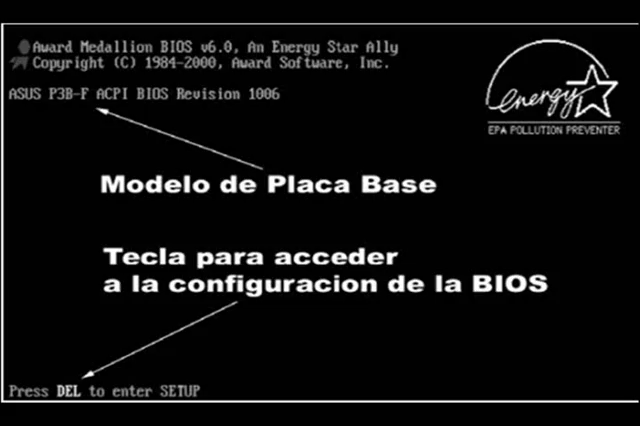
\includegraphics[scale=0.6]{presentacion/Screenshot-Ingresando_al_BIOS_Setup-1.png}
		\caption{El BIOS al encender la computadora.}
	\end{figure}

	Cuando se acciona el botón de encendido o se presiona el botón de re-inicio
	(Reset) la carga eléctrica inicial hace que arranque la unidad central de
	% Fix accents
	proceso y pide instrucciones al BIOS (instrucciones permanentes que no se
	borran al apagar la computadora). 
	\\ 
	El CPU empieza a ejecutar las instrucciones, en particular la Auto prueba
	de arranque (Power On Self Test, POST) la cual verifica la integridad de la
	memoria, controladores, y dispositivos del sistema. 
	\\ 
	Actualmente el sistema de Conectar y Funcionar (Plug and Play) es muy
	común, por lo que hay que evaluar la memoria de acceso aleatorio (Random
	Access Memory, RAM), configurar los adaptadores de Conectar y Funcionar, el 
	sonido y el vídeo. 
	\\ 
	Si el BIOS no es de Conectar y Funcionar, el arranque del sistema pasa a la
	siguiente fase. 
	\\ 
	El BIOS busca un disco de arranque con las instrucciones para cargar el
	sistema operativo.  Típicamente el BIOS busca primero en la unidad A: y
	luego en la unidad C: hasta que halla el disco de arranque y lee el primer
	sector o bloque de información. Este es el sector de arranque que contiene
	las instrucciones para cargar el sistema operativo.

	%\subsection{Solución de problemas}{\label{sec:bios/solucion-de-problemas}}
		%\subsubsection{Pitidos de la BIOS (Award)}{\label{sec:bios/tonos-de-la-bios}}

		%En esta seccion cubriremos los significados de los pitidos de los BIOS {\em Award}. \\
		%En la mayoría de los pitidos se les acompaña un mensaje de error. 

			%\paragraph{Tono ininterrumpido}:
			
			%Fallo en el suministro elctrico. Revisamos las conexiones y la fuente
			%de alimentación.  Tonos cortos constantes: Sobrecarga elctrica, chips
			%defectuosos, placa mal.

			%\paragraph{1 largo}:

			%Si aparece esto en la pantalla “RAM Refresh Failure”, significa que los
			%diferentes componentes encargados del refresco de la memoria RAM fallan
			%o no están presentes. Cambiar de banco la memoria y comprobar los
			%jumpers de buses. 

			%\paragraph{1 largo y 1 corto}: 

			%El código de la BIOS esta corrupto o defectuoso, probaremos a flasear o
			%reemplazamos el chip de la BIOS sino podemos cambiamos de placa. 

			%\paragraph{1 largo y dos cortos}:
			
			%No da señal de imagen, se trata de que nuestra tarjeta de vídeo esta
			%estropeada, probaremos a pincharla en otro slot o probaremos otra
			%tarjeta gráfica. 

			%\paragraph{1 largo y 2 cortos}:

			%Si aparece por pantalla este mensaje: “No video card found”, este error
			%solo es aplicable a placas base con tarjetas de vídeo integradas. Fallo
			%en la tarjeta gráfica, probaremos a deshabilitarla y pincharemos una
			%nueva en cualquier slot libre o cambiaremos la placa madre. 

			%\paragraph{1 largo y 3 cortos}:

			%Si aparece este mensaje por pantalla “No monitor connected” Idem que el
			%anterior. 

			%\paragraph{1 largo y varios cortos}: 

			%Mensaje de error. “Video related failure”. Lo mismo que antes. Cada
			%fabricante implanta un código de error según el tipo de tarjeta de
			%video y los parámetros de cada BIOS.

			%\paragraph{2 largos y 1 corto}:
			
			%Fallo en la sincronización de las imágenes. Cargaremos por defecto los
			%valores de la BIOS e intentaremos reiniciar. Si persiste nuestra
			%tarjeta gráfica o placa madre están estropeadas. 

			%\paragraph{2 cortos}:
			
			%Vemos en la pantalla este error: “Parity Error”. Se trata de un error
			%en la configuración de la BIOS al no soportar la paridad de memoria, la
			%deshabilitamos en al BIOS. 

			%\paragraph{3 cortos}:
			
			%Vemos en la pantalla este error. Base 64 Kb “Memory Failure”, significa
			%que la BIOS al intentar leer los primeros 64Kbytes de memoria RAM
			%dieron error. Cambiamos la RAM instalada por otra. 

			%\paragraph{4 cortos}:
			
			%Mensaje de error; “Timer not operational”. El reloj de la propia placa
			%base esta estropeado, no hay más solución que cambiar la placa. No
			%confundir con “CMOS cheksum error” una cosa es la pila y otra el
			%contador o reloj de la placa base. 

			%\paragraph{5 cortos}:
			
			%Mensaje por pantalla ``Processor Error'' significa que la CPU ha generado
			%un error porque el procesador o la memoria de vídeo están bloqueados. 

			%\paragraph{6 cortos}:

			%Mensaje de error: ``8042 - Gate A20 Failure'', muy mítico este error.
			%El controlador o procesador del teclado (8042) puede estar en mal
			%estado. 
			%La BIOS no puede conmutar en modo protegido. Este error se
			%suele dar cuando se conecta/desconecta el teclado con el ordenador
			%encendido. 

			%\paragraph{7 cortos}:
			
			%Mensaje de error: “Processor Exception / Interrupt Error” Descripción. La CPU ha generado una interrupción excepcional o el modo virtual del procesador está activo. Procesador a punto de morirse. 

			%\paragraph{8 cortos}:
			
			%Mensaje de error: ``Display Memory Read / Write error''. La tarjeta de video esta estropeada, procedemos a cambiarla. 

			%\paragraph{9 cortos}:
			
			%Mensaje de error: ``ROM Checksum Error''; el valor del checksum (conteo de la memoria) de la RA

		%\newpage

		%\subsubsection{Errores en pantalla}\label{sub:errores en pantalla}
		
		%Los siguientes errores de pantalla son errores generales o bien, no dependen de marca y modelo de la BIOS:

			%\paragraph{BIOS ROM checksum error – system halted}

			%El código de control de la BIOS es incorrecto, lo que indica que puede
			%estar corrupta. En caso de reiniciar y repetir el mensaje, tendremos
			%que reemplazar al BIOS.

			%\paragraph{CMOS battery failed}

			%La pila de la placa base que alimenta la memoria CMOS ha dejado de
			%suministrar corriente. Es necesario cambiar la pila inmediatamente.

			%\paragraph{CMOS checksum error – Defaults loaded}

			%El código de control de la CMOS no es correcto, por lo que se
			%procede a cargar los parámetros de la BIOS por defecto. Este error
			%se produce porque la información almacenada en la CMOS es
			%incorrecta, lo que puede indicar que la pila está empezando a
			%fallar.

			%\paragraph{Display switch is set incorrectly}

			%El tipo de pantalla especificada en la BIOS es incorrecta. Esto puede ocurrir si hemos seleccionado la existencia de un adaptador monocromo cuando tenemos uno en color, o al contrario. Bastará con poner bien este parámetro para solucionar el problema.

			%\paragraph{Floppy disk(s) Fail} 
			
			%(code 40/38/48 dependiendo de la antigüedad de la bios)

			%Disquetera mal conectada, verificamos todos los cables de conexión.

			%\paragraph{Hard disk install failure}

			%La BIOS no es capaz de inicializar o encontrar el disco duro de
			%manera correcta. Debemos estar seguros de que todos de que todos
			%los discos se encuentren bien conectados y correctamente
			%configurados.

			%\paragraph{Keyboard error or no keyboard present}

			%No es posible inicializar el teclado. Puede ser debido a que no se
			%encuentre conectado, este estropeado e incluso porque mantenemos
			%pulsada alguna tecla durante el proceso de arranque.

			%\paragraph{Keyboard error is locked out – Unlock the key}

			%Este mensaje solo aparece en muy pocas BIOS, cuando alguna tecla ha
			%quedado presionada. 

			%\paragraph{Memory Test Fail}

			%El chequeo de memoria RAM ha fallado debido probablemente, a
			%errores en los módulos de memoria. En caso de que nos aparezca este
			%mensaje, hemos de tener mucha precaución con el equipo, se puede
			%volver inestable y tener prdidas de datos. Solución, comprobar que
			%banco de memoria está mal, y sustituirlo inmediatamente. 

			%\paragraph{Override enabled – Defaults loaded}

			%Si el sistema no puede iniciarse con los valores almacenados en la
			%CMOS, la BIOS puede optar por sustituir estos por otros genricos
			%diseñados para que todo funcione de manera estable, aunque sin
			%obtener las mayores prestaciones. 

			%\paragraph{Primary master hard diskfail}

			%El proceso de arranque ha detectado un fallo al iniciar el disco
			%colocado como maestro en el controlador IDE primario. Para
			%solucionar comprobaremos las conexiones del disco y la
			%configuración de la BIOS. 
	

	\newpage
\section{El CMOS Setup}{\label{sec:cmossetup}}

	El CMOS Setup es un conjunto de instrucciones en la BIOS que permite
	manipular la información en los chips CMOS.

	{\bf Recordar:} El BIOS es de solo lectura; el CMOS chip es de escritura/lectura.

	El CMOS requiere de energía eléctrica constante para no perder la
	información guardada en los chips CMOS y por eso los fabricantes de las
	placas madres lo traen con una pila de bajo voltaje y consumo.

	La pila se recarga automáticamente al encender la computadora y puede
	provenir la capacidad suficiente para aproximadamente 1000 días.

	Según la marca de BIOS, puede tratarse de la tecla F2, de la tecla F10, o
	bien de la tecla Supr, o alguna de las siguientes secuencias de teclas: 

	\begin{verbatim}
	Ctrl + Alt + S 
	Ctrl + Alt + Esc 
	Ctrl + Alt + Ins 
	\end{verbatim}

	En los BIOS Award, se muestran los siguientes mensajes durante el POST:
	PARA INGRESAR A LA CONFIGURACIÓN ANTES DE REINICIAR PRESIONE CTRL-ALT-ESC O LA TECLA DEL

	\newpage
	\subsection{Pantallas en el CMOS Setup}{\label{sub:pantallas en el cmos setup}}

		\subsubsection{Pantalla Principal}{\label{sub:pantalla principal}}
			\begin{figure}[H]
				\centering
					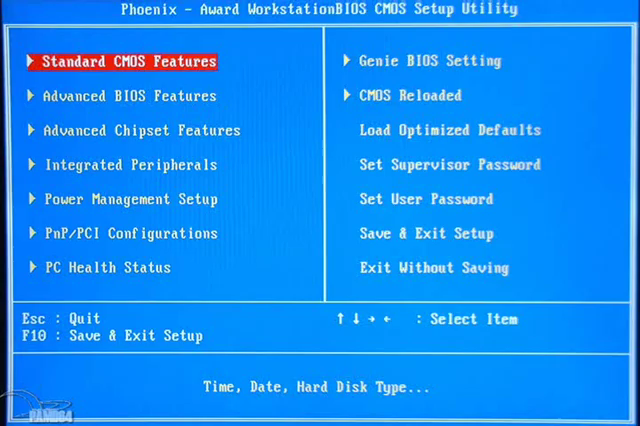
\includegraphics[scale=0.6]{presentacion/00.png}
				\caption{La pantalla principal del CMOS Setup.}
			\end{figure}

		\subsubsection{Standard CMOS Setup}{\label{sub:Standard cmos setup}}
			\begin{figure}[H]
				\centering
					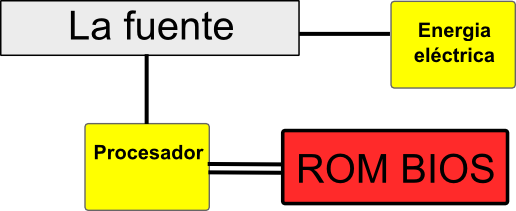
\includegraphics[scale=0.5]{presentacion/01.png}
				\caption{La pantalla del ``Standard CMOS Setup''.}
			\end{figure}

		\subsubsection{BIOS Features Setup}{\label{sub:bios features setup}}
			\begin{figure}[H]
				\centering
					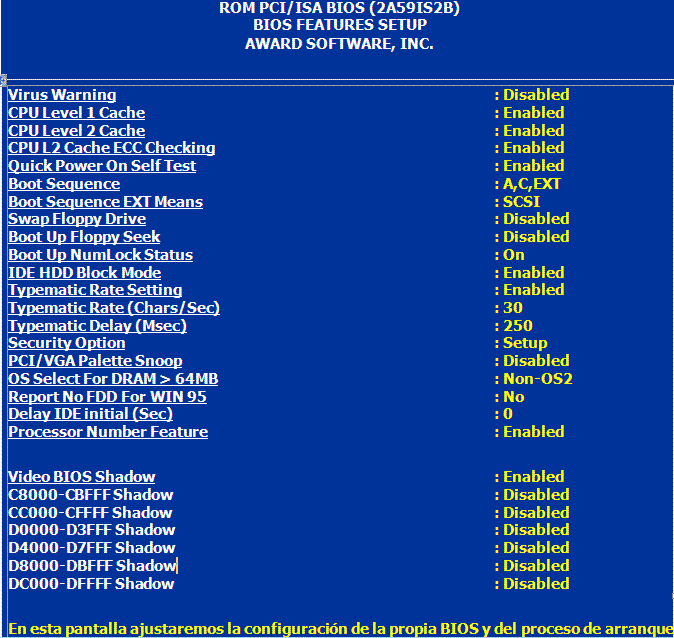
\includegraphics[scale=0.5]{presentacion/02.png}
				\caption{``BIOS Features Setup''}
			\end{figure}

			\paragraph{CPU Level 1\&2 Cache}
			Activa o desactiva la cache de primer y segundo nivel integrada en
			el núcleo del procesador.
			\paragraph{Boot Sequence}
			Indica el orden de búsqueda de la unidad en la que arrancará el
			sistema operativo.
			\paragraph{Boot Up NumLock Status}
			En ``ON'', la BIOS activa automáticamente la tecla ``NumLock'' del
			teclado numérico en el proceso de arranque.

		
		\subsubsection{Chipset Features Setup}{\label{sub:chipset features setup}}
			\begin{figure}[H]
				\centering
					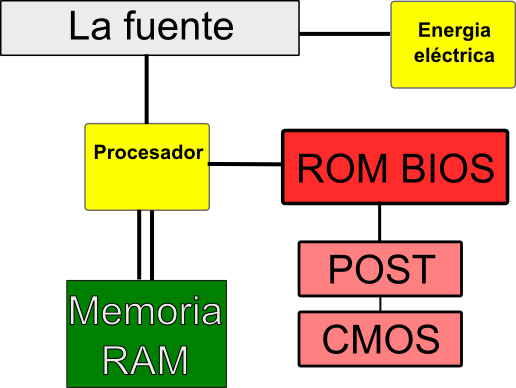
\includegraphics[scale=0.5]{presentacion/03.png}
				\caption{``Chipset Features Setup''.}
			\end{figure}

		\subsubsection{Power Management Setup}{\label{sub:power management setup}}
			\begin{figure}[H]
				\centering
					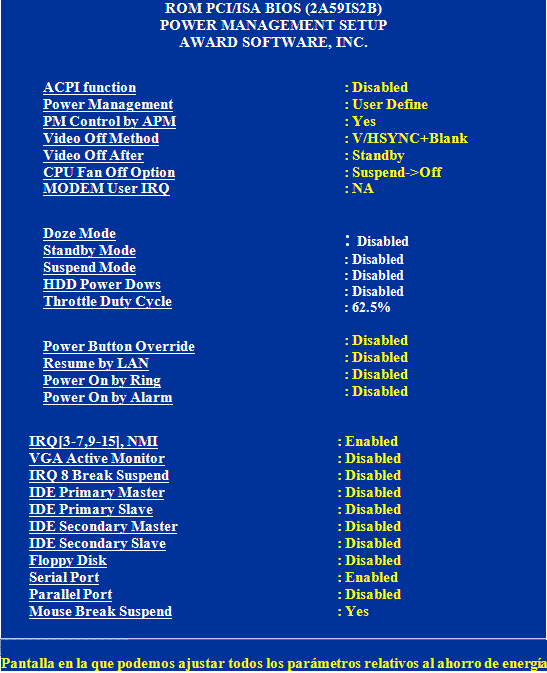
\includegraphics[scale=0.5]{presentacion/04.png}
				\caption{``Power Management Setup''.}
			\end{figure}

		\subsubsection{PNP/PCI Configuration}{\label{sub:pnp/pci configuration}}
			\begin{figure}[H]
				\centering
					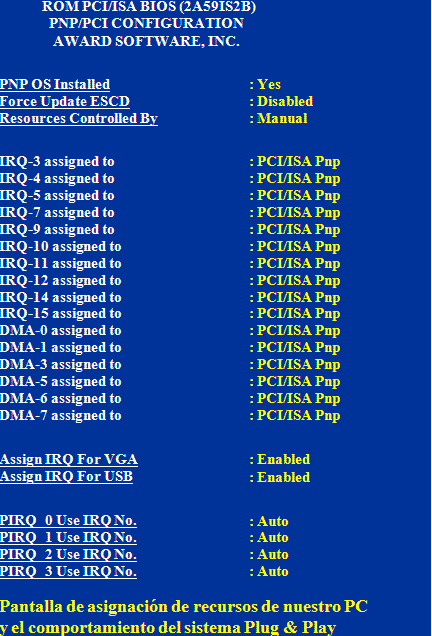
\includegraphics[scale=0.5]{presentacion/05.png}
				\caption{``Configuracion de PNP/PCI''.}
			\end{figure}

		\newpage

	\subsection{Restaurar la configuración del CMOS Setup}{\label{sec:cmossetup/resetear-el-cmos-setup}}

	Hay varias formas de restaurar la configuración del CMOS Setup o bien del chip CMOS.

	Generalmente no se lo hace, pero en caso de olvidar la contraseña de acceso al CMOS Setup un reseteo sera inevitable.

	\subsubsection{Metodo 1}{\label{sec:metodo 1}}

	Sacar la pila del CMOS que se encuentra sujetada en un slot para la pila en
	la placa base por unos segundos, despues reemplazarla otravez.

	\subsubsection{Metodo 2}{\label{sec:metodo 2}}

	Algunas placas base ofrecen un jumper CMOS-reset o un botón de reinicio.



	\subsubsection{Metodo 3}{\label{sec:metodo 3}}

	En otros casos, el chip EEPROM ha de desoldar los datos en forma manual,
	por manos de un programador. A veces es suficiente motivo para el CLK o
	línea de DTA de la I2C bus de la EEPROM en el momento adecuado durante el
	arranque, esto requiere una cierta precisión en las piezas de soldadura
	SMD. Si la máquina le permite arrancar, pero no quiere que le permiten a la
	configuración de la BIOS, una posible recuperación es dañar la suma de
	comprobación CMOS, haciendo puerto directo escribe usando debug.exe,
	corrompiendo a algunos bytes de la suma de control de área protegida de la
	RAM CMOS, en el siguiente arranque, el equipo normalmente restablece su
	configuración de fábrica. Por ejemplo:

	\begin{verbatim}
	c:\debug
	-o 70 10
	-o 71 aa
	-q
	\end{verbatim}

	Que permitirá escribir en CMOS (Offset 10h) con el valor 0AAhA.

	\newpage

\begin{thebibliography}{9}{\label{sec:bibliografia}}

	\bibitem{WIC}
		What is CMOS?,
		\url{http://www.wisegeek.com/what-is-cmos.htm}

	\bibitem{UnidadIIBIOSExposicion.ppt}
		% CORREGIR!
		Exposicion de BIOS de la Universidad BLABLA

	\bibitem{BIOS}
		``BIOS'' - {\em Basic Input-Output System}
		\url{http://es.wikipedia.org/wiki/BIOS}

	\bibitem{CIL}
		Dan Clein, ``CMOS IC LAYOUT Concepts, Methodologies, and Tools'', pp. 22 - 26, 2000

	\bibitem{MDB}
		Mesmer, ``Manual de la BIOS'', Marzo 2001
	
	\bibitem{BootProcess}
		\url{http://duartes.org/gustavo/blog/post/how-computers-boot-up/}

\end{thebibliography}
\end{document}
